% Provenance: Grashopr-888/ISMIR_LBD_2026@2bf21d1:paper/figures/fig_system_i0.tex (changed: panel C draws Elk's image only if present; it is not redistributed)
% Figure 1 of the paper: the latent granular instrument offline (A) and on the Elk Stomp (B), and the board (C).
% Build: cd figures && tectonic fig_system.tex   (any LaTeX with TikZ and standalone works)
% Drawn at the printed width (one ISMIR column, 82 mm = 232.4 pt), so the 6.2 pt box text and 7 pt panel titles
% print at their own size (the paper includes the PDF at \columnwidth, scale about 1.0).
% Greyscale-safe: panel A has a grey fill, panel B none, the worker thread a dashed outline, and the two student
% boxes share the one accent fill (light orange, grey level about 0.85 against 1.0 for the white boxes).
% Facts drawn: analysis every 4,480 samples = 93.3 ms on a worker thread, audio callback 64 samples = 1.333 ms,
% the pack, mel-latent pairs; front-end = resampling, 4096-point FFT, 80 log-mel bands (results/board/README.md).
% Panel C: elk_stomp_board_i0.jpg, a crop of Elk's render of the board (Elk's desktop-devkit README) with
% the shadows lifted (gamma 0.62, contrast 1.12) so it reads in greyscale. Credit in the caption: "Image: Elk Audio."
\documentclass[tikz,border=0.4pt]{standalone}
\usetikzlibrary{arrows.meta,positioning,calc}
\definecolor{accent}{RGB}{250,214,176}
\begin{document}
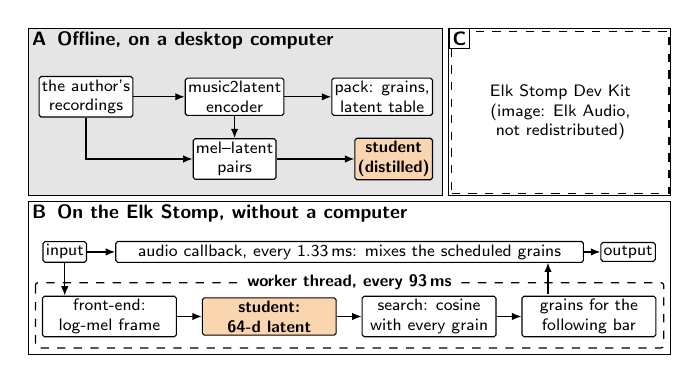
\begin{tikzpicture}[x=1mm,y=1mm,font=\sffamily\fontsize{6.2}{7.1}\selectfont,
  box/.style={draw,line width=0.4pt,rounded corners=0.7pt,inner xsep=1.0pt,inner ysep=1.1pt,align=center,fill=white},
  stu/.style={box,fill=accent,font=\sffamily\bfseries\fontsize{6.2}{7.1}\selectfont},
  panel/.style={draw,line width=0.45pt},
  lab/.style={font=\sffamily\bfseries\fontsize{7}{8}\selectfont,anchor=north west,inner sep=1.2pt},
  arr/.style={-{Latex[length=1.2mm,width=0.95mm]},line width=0.5pt}]

% ---------------- Panel A: offline, on a desktop computer ----------------
\fill[black!10] (0,0) rectangle (52.6,-21.2);
\draw[panel] (0,0) rectangle (52.6,-21.2);
\node[lab] at (0,0) {A\enspace Offline, on a desktop computer};
\node[box,anchor=west] (rec) at (1.3,-8.7) {the author's\\recordings};
\node[box] (enc) at (26.2,-8.7) {music2latent\\encoder};
\node[box,anchor=east] (pack) at (51.4,-8.7) {pack: grains,\\latent table};
\draw[arr] (rec) -- (enc); \draw[arr] (enc) -- (pack);
\node[box] (pairs) at (26.2,-16.6) {mel--latent\\pairs};
\node[stu,anchor=east] (stuA) at (51.4,-16.6) {student\\(distilled)};
\draw[arr] (enc) -- (pairs);
\draw[arr] (rec.south) |- (pairs.west);
\draw[arr] (pairs) -- (stuA);

% ---------------- Panel C: the board ----------------
\draw[panel] (53.4,0) rectangle (81.6,-21.2);
% Elk Audio's render of the board is third-party and not in this repository: put your own copy next to this
% file as elk_stomp_board_i0.jpg to reproduce the paper's panel C, otherwise a labelled frame is drawn.
\IfFileExists{elk_stomp_board_i0.jpg}
  {\node[anchor=north west,inner sep=0pt] (img) at (53.7,-0.3) {\includegraphics[width=27.6mm,height=20.6mm]{elk_stomp_board_i0.jpg}};}
  {\node[anchor=north west,inner sep=0pt,draw,dashed,minimum width=27.6mm,minimum height=20.6mm,align=center] (img) at (53.7,-0.3) {Elk Stomp Dev Kit\\(image: Elk Audio,\\not redistributed)};}
\node[lab,fill=white,draw=black,line width=0.3pt] at (53.4,0) {C};

% ---------------- Panel B: on the Elk Stomp ----------------
\draw[panel] (0,-22.0) rectangle (81.6,-41.4);
\node[lab] at (0,-22.0) {B\enspace On the Elk Stomp, without a computer};
\node[box,anchor=west] (in) at (1.8,-28.4) {input};
\node[box,anchor=east] (out) at (79.7,-28.4) {output};
\node[box,minimum width=59.4mm] (cb) at (40.8,-28.4) {audio callback, every 1.33\,ms: mixes the scheduled grains};
\draw[arr] (in) -- (cb); \draw[arr] (cb) -- (out);
% worker thread: four equal boxes, 17 mm wide, centres 20.3 mm apart
\draw[line width=0.45pt,dashed,rounded corners=1pt] (0.9,-32.3) rectangle (80.7,-40.6);
\node[fill=white,inner sep=0.8pt,font=\sffamily\bfseries\fontsize{6.2}{7.1}\selectfont] at (40.8,-32.3) {worker thread, every 93\,ms};
\node[box,minimum width=17mm] (fe) at (10.3,-36.6) {front-end:\\log-mel frame};
\node[stu,minimum width=17mm] (stuB) at (30.6,-36.6) {student:\\64-d latent};
\node[box,minimum width=17mm] (se) at (50.9,-36.6) {search: cosine\\with every grain};
\node[box,minimum width=17mm] (sch) at (71.2,-36.6) {grains for the\\following bar};
\draw[arr] (fe) -- (stuB); \draw[arr] (stuB) -- (se); \draw[arr] (se) -- (sch);
\draw[arr] (in.south) -- (in.south |- fe.north);
\draw[arr] (66.0,-33.7) -- (66.0,-29.75);
\end{tikzpicture}
\end{document}
